\documentclass{standalone}
\usepackage{tikz}
\usetikzlibrary{patterns, positioning}
\usepackage[sfdefault]{ClearSans} %% option 'sfdefault' activates Clear Sans as the default text font
\usepackage[T1]{fontenc}

\begin{document}
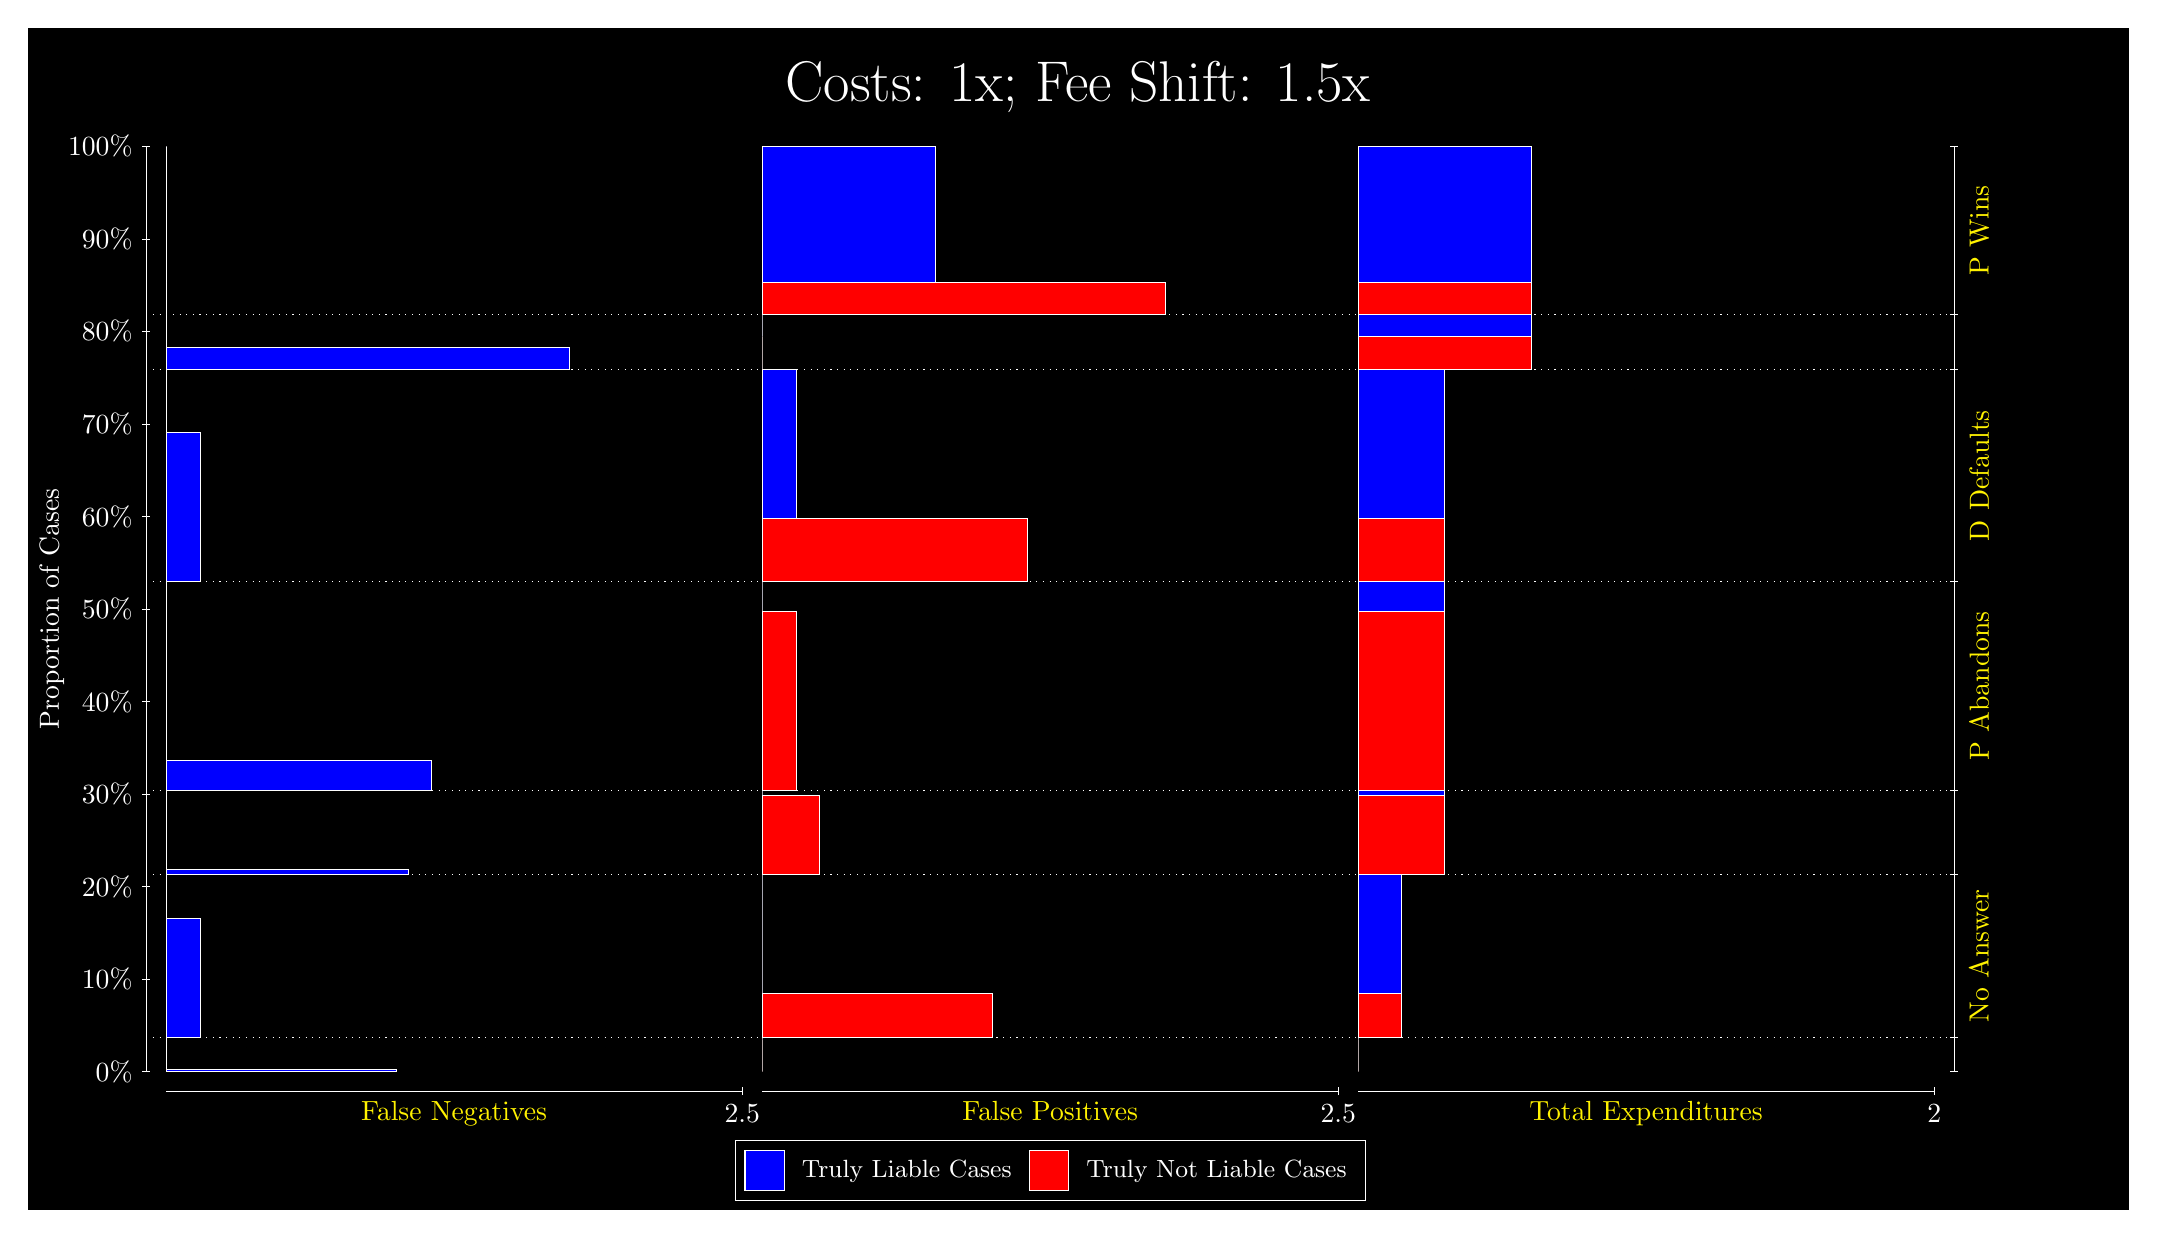
\begin{tikzpicture}
\draw[fill=black] (0,0) rectangle (26.667,15);
\draw[text=white] (0,13.5) rectangle (26.667,15) node[midway] {\huge Costs: 1x; Fee Shift: 1.5x};
\draw[white, very thin] (1.5,1.75) -- (1.5,13.5);
\node[rotate=90, text=white, anchor=center] at (0.3, 7.625) {Proportion of Cases};
\draw[white, very thin] (1.45,1.75) -- (1.55,1.75);
\node[text=white, anchor=east] at (1.45, 1.75) {0\%};
\draw[white, very thin] (1.45,2.925) -- (1.55,2.925);
\node[text=white, anchor=east] at (1.45, 2.925) {10\%};
\draw[white, very thin] (1.45,4.1) -- (1.55,4.1);
\node[text=white, anchor=east] at (1.45, 4.1) {20\%};
\draw[white, very thin] (1.45,5.275) -- (1.55,5.275);
\node[text=white, anchor=east] at (1.45, 5.275) {30\%};
\draw[white, very thin] (1.45,6.45) -- (1.55,6.45);
\node[text=white, anchor=east] at (1.45, 6.45) {40\%};
\draw[white, very thin] (1.45,7.625) -- (1.55,7.625);
\node[text=white, anchor=east] at (1.45, 7.625) {50\%};
\draw[white, very thin] (1.45,8.8) -- (1.55,8.8);
\node[text=white, anchor=east] at (1.45, 8.8) {60\%};
\draw[white, very thin] (1.45,9.975) -- (1.55,9.975);
\node[text=white, anchor=east] at (1.45, 9.975) {70\%};
\draw[white, very thin] (1.45,11.15) -- (1.55,11.15);
\node[text=white, anchor=east] at (1.45, 11.15) {80\%};
\draw[white, very thin] (1.45,12.325) -- (1.55,12.325);
\node[text=white, anchor=east] at (1.45, 12.325) {90\%};
\draw[white, very thin] (1.45,13.5) -- (1.55,13.5);
\node[text=white, anchor=east] at (1.45, 13.5) {100\%};

\draw[white, very thin] (24.457,1.75) -- (24.457,13.5);
\draw[white, very thin] (24.407,1.75) -- (24.507,1.75);
\node[anchor=west] at (24.407, 1.75) {};
\draw[white, very thin] (24.407,2.1824) -- (24.507,2.1824);
\node[anchor=west] at (24.407, 2.1824) {};
\draw[white, very thin] (24.407,4.2568) -- (24.507,4.2568);
\node[anchor=west] at (24.407, 4.2568) {};
\draw[white, very thin] (24.407,5.3219) -- (24.507,5.3219);
\node[anchor=west] at (24.407, 5.3219) {};
\draw[white, very thin] (24.407,7.974) -- (24.507,7.974);
\node[anchor=west] at (24.407, 7.974) {};
\draw[white, very thin] (24.407,10.663) -- (24.507,10.663);
\node[anchor=west] at (24.407, 10.663) {};
\draw[white, very thin] (24.407,11.365) -- (24.507,11.365);
\node[anchor=west] at (24.407, 11.365) {};
\draw[white, very thin] (24.407,13.5) -- (24.507,13.5);
\node[anchor=west] at (24.407, 13.5) {};

\draw[white, very thin, fill=blue] (1.75,1.75) rectangle (4.6775,1.7753);
\draw[white, very thin, fill=red] (1.75,1.7753) rectangle (1.75,2.1824);
\draw[white, very thin, fill=blue] (1.75,2.1824) rectangle (2.1891,3.6986);
\draw[white, very thin, fill=red] (1.75,3.6986) rectangle (1.75,4.2568);
\draw[white, very thin, fill=blue] (1.75,4.2568) rectangle (4.8239,4.3184);
\draw[white, very thin, fill=red] (1.75,4.3184) rectangle (1.75,5.3219);
\draw[white, very thin, fill=blue] (1.75,5.3219) rectangle (5.1167,5.6972);
\draw[white, very thin, fill=red] (1.75,5.6972) rectangle (1.75,7.974);
\draw[white, very thin, fill=blue] (1.75,7.974) rectangle (2.1891,9.8667);
\draw[white, very thin, fill=red] (1.75,9.8667) rectangle (1.75,10.663);
\draw[white, very thin, fill=blue] (1.75,10.663) rectangle (6.8732,10.943);
\draw[white, very thin, fill=red] (1.75,10.943) rectangle (1.75,11.365);
\draw[white, very thin, fill=red] (1.75,11.365) rectangle (1.75,11.776);
\draw[white, very thin, fill=blue] (1.75,11.776) rectangle (1.75,13.5);
\draw[white, very thin, fill=red] (9.3189,1.75) rectangle (9.3189,2.1571);
\draw[white, very thin, fill=blue] (9.3189,2.1571) rectangle (9.3189,2.1824);
\draw[white, very thin, fill=red] (9.3189,2.1824) rectangle (12.246,2.7406);
\draw[white, very thin, fill=blue] (9.3189,2.7406) rectangle (9.3189,4.2568);
\draw[white, very thin, fill=red] (9.3189,4.2568) rectangle (10.051,5.2603);
\draw[white, very thin, fill=blue] (9.3189,5.2603) rectangle (9.3189,5.3219);
\draw[white, very thin, fill=red] (9.3189,5.3219) rectangle (9.758,7.5987);
\draw[white, very thin, fill=blue] (9.3189,7.5987) rectangle (9.3189,7.974);
\draw[white, very thin, fill=red] (9.3189,7.974) rectangle (12.686,8.7702);
\draw[white, very thin, fill=blue] (9.3189,8.7702) rectangle (9.758,10.663);
\draw[white, very thin, fill=red] (9.3189,10.663) rectangle (9.3189,11.085);
\draw[white, very thin, fill=blue] (9.3189,11.085) rectangle (9.3189,11.365);
\draw[white, very thin, fill=red] (9.3189,11.365) rectangle (14.442,11.776);
\draw[white, very thin, fill=blue] (9.3189,11.776) rectangle (11.515,13.5);
\draw[white, very thin, fill=red] (16.888,1.75) rectangle (16.888,2.1571);
\draw[white, very thin, fill=blue] (16.888,2.1571) rectangle (16.888,2.1824);
\draw[white, very thin, fill=red] (16.888,2.1824) rectangle (17.437,2.7406);
\draw[white, very thin, fill=blue] (16.888,2.7406) rectangle (17.437,4.2568);
\draw[white, very thin, fill=red] (16.888,4.2568) rectangle (17.986,5.2603);
\draw[white, very thin, fill=blue] (16.888,5.2603) rectangle (17.986,5.3219);
\draw[white, very thin, fill=red] (16.888,5.3219) rectangle (17.986,7.5987);
\draw[white, very thin, fill=blue] (16.888,7.5987) rectangle (17.986,7.974);
\draw[white, very thin, fill=red] (16.888,7.974) rectangle (17.986,8.7702);
\draw[white, very thin, fill=blue] (16.888,8.7702) rectangle (17.986,10.663);
\draw[white, very thin, fill=red] (16.888,10.663) rectangle (19.083,11.085);
\draw[white, very thin, fill=blue] (16.888,11.085) rectangle (19.083,11.365);
\draw[white, very thin, fill=red] (16.888,11.365) rectangle (19.083,11.776);
\draw[white, very thin, fill=blue] (16.888,11.776) rectangle (19.083,13.5);
\draw[white, dotted] (1.5,2.1824) -- (24.457,2.1824);
\draw[white, dotted] (1.5,4.2568) -- (24.457,4.2568);
\draw[white, dotted] (1.5,5.3219) -- (24.457,5.3219);
\draw[white, dotted] (1.5,7.974) -- (24.457,7.974);
\draw[white, dotted] (1.5,10.663) -- (24.457,10.663);
\draw[white, dotted] (1.5,11.365) -- (24.457,11.365);
\draw[white, very thin] (1.75,1.5) -- (9.0689,1.5);
\node[text=yellow, anchor=north] at (5.4094, 1.5) {False Negatives};
\draw[white, very thin] (9.0689,1.45) -- (9.0689,1.55);
\node[text=white, anchor=north] at (9.0689, 1.45) {2.5};

\draw[white, very thin] (9.3189,1.5) -- (16.638,1.5);
\node[text=yellow, anchor=north] at (12.978, 1.5) {False Positives};
\draw[white, very thin] (16.638,1.45) -- (16.638,1.55);
\node[text=white, anchor=north] at (16.638, 1.45) {2.5};

\draw[white, very thin] (16.888,1.5) -- (24.207,1.5);
\node[text=yellow, anchor=north] at (20.547, 1.5) {Total Expenditures};
\draw[white, very thin] (24.207,1.45) -- (24.207,1.55);
\node[text=white, anchor=north] at (24.207, 1.45) {2};


\node[text=yellow, centered, rotate=90] at (24.777, 3.2196) {No Answer};

\node[text=yellow, centered, rotate=90] at (24.777, 6.648) {P Abandons};
\node[text=yellow, centered, rotate=90] at (24.777, 9.3185) {D Defaults};

\node[text=yellow, centered, rotate=90] at (24.777, 12.432) {P Wins};

\draw (12.978300999999998,1.5) node[draw=none] (baseCoordinate) {};
\begin{scope}[align=center]
        \matrix[scale=0.5, draw=white, below=0.5cm of baseCoordinate, nodes={draw}, column sep=0.1cm]{
            \node[rectangle, draw, minimum width=0.5cm, minimum height=0.5cm, fill=blue] {}; &
            \node[draw=none, font=\small, text=white] (B) {Truly Liable Cases}; &
            \node[rectangle, draw, minimum width=0.5cm, minimum height=0.5cm, fill=red] {}; &
            \node[draw=none, font=\small, text=white] (B) {Truly Not Liable Cases}; \\
            };
\end{scope}

\end{tikzpicture}
\end{document}